% File: main.tex
% Target Journal: International Journal of Artificial Intelligence in Education (IJAIED)
% Style: Elsevier template format (elsarticle - numeric style)

\documentclass[final,5p,times,twocolumn,authoryear]{elsarticle}

\usepackage{amsmath,amssymb,amsfonts}
\usepackage{graphicx}
\usepackage{url}
\usepackage{hyperref}
\usepackage{booktabs}
\usepackage{microtype}
\usepackage{enumitem}

\journal{International Journal of Artificial Intelligence in Education}

\begin{document}

\begin{frontmatter}

\title{Closed-Loop State-Sensing Intelligent Tutoring Architecture for Personalized Multimodal Education}
\author[inst1]{Dr. Richa Sharma}
\ead{richa@example.com}
\address[inst1]{Department of Computer Science and Engineering}
\author[inst2]{A. R. Keerthana}
\ead{keerthana@example.com}
\address[inst2]{Department of Computer Science and Engineering}

\begin{abstract}
Traditional digital educational platforms adopt a static, one-size-fits-all approach that fails to accommodate the cognitive, affective, and sensory requirements of neurodivergent learners. This paper presents a novel closed-loop, state-sensing Intelligent Tutoring System (ITS) that dynamically estimates learner focus, behavioral impatience, and concept mastery to personalize content delivery in real-time. By integrating edge-based gaze tracking (analyzing facial landmarks at $1\text{ Hz}$ via OpenCV and dlib) with micro-interaction telemetry, the system detects distraction and frustration without harvesting sensitive biometric video data. Sensory accommodations and content adaptations are resolved using a deterministic priority hierarchy in a Neo4j Knowledge Graph, prioritizing clinical disability accommodations (ADHD, Autism Spectrum Disorder, Dyslexia) over inferred behavioral preferences and manual user selections. The adaptive content generation engine leverages Retrieval-Augmented Generation (RAG) and Llama 3 to compile explanations into dynamic Mermaid.js flowcharts, Text-to-Speech audio streams, and MoviePy-synthesized educational video lessons. Active comprehension is verified via RAG-driven quizzes and speech-to-text active recall evaluation. Empirical database verification confirms the real-time stability of exponential moving average (EMA) concept mastery trajectories and programmatic behavioral reinforcement loops. This architecture establishes a scalable, privacy-preserving paradigm for equitable, adaptive education.
\end{abstract}

\begin{keyword}
Generative AI \sep Intelligent Tutoring Systems \sep Neurodiversity \sep Affective Computing \sep Universal Design for Learning \sep Knowledge Graphs \sep Multimodal Learning
\end{keyword}

\end{frontmatter}

\section{Introduction}
\label{sec:introduction}

The emergence of Large Language Models (LLMs) and generative artificial intelligence (GenAI) has transformed Intelligent Tutoring Systems (ITSs) by allowing real-time, conversational explanations tailored to user queries. However, standard GenAI tutoring interfaces operate in an affective and cognitive vacuum. Although they can adjust their lexical complexity, they lack sensory channels to detect a student's real-time engagement, cognitive load, or frustration. Consequently, they deliver explanations in a uniform, text-dense format. This lack of sensory feedback presents a significant barrier for neurodivergent learners (such as those with ADHD, Autism, or dyslexia) and students experiencing learning-induced anxiety, who require active cognitive pacing and multi-sensory formats.

To bridge this gap, this paper presents a closed-loop, state-sensing GenAI tutoring architecture that continuously estimates a learner's cognitive, physical, and emotional states during a study session. The system implements a strict priority hierarchy that balances medical, behavioral, and manual student inputs to resolve content delivery. By capturing real-time gaze indicators via webcam, sensing user impatience through interaction telemetry, and managing historical mastery data within a Neo4j Knowledge Graph, the system dynamically adapts its pedagogical delivery. Rather than relying on black-box neural reinforcement learning, which poses unpredictable behaviors in educational settings, the system implements a programmatic graph-based feedback loop. This loop dynamically translates educational content into optimal formats—including structured Mermaid.js diagrams, synthesized audio, and custom-generated educational videos—pacing the material to suit the individual student's profile.

\subsection{Background and Motivation}
\label{subsec:bg_motivation}

Standard e-learning platforms rely on static text, which often introduces high cognitive load and orthographic barriers. A cornerstone of this architecture is its strict adherence to scientifically backed pedagogical frameworks for neurodivergent learners:
\begin{itemize}
    \item \textbf{Attention-Deficit/Hyperactivity Disorder (ADHD):} Rooted in the Universal Design for Learning (UDL) framework and Cognitive Load Theory \cite{2}, students with ADHD benefit from reducing extraneous cognitive load. The system limits the number of concepts introduced at once, structures text using bullet points, and defaults to high-stimulation modalities (Videos or Diagrams) for severe cases to break content into manageable, dopamine-rewarding chunks \cite{15}.
    \item \textbf{Autism Spectrum Disorder (ASD):} Guided by Visual Support Theory and research into central coherence in ASD, autistic learners often possess strong visual-spatial processing skills but struggle with abstract linguistic concepts or implicit social context \cite{13, 16}. The system enforces structured explanations, explicit step-by-step logic, and strictly avoids metaphors or ambiguous idioms, leaning heavily on visual Mermaid.js flowcharts to make conceptual relationships explicit and unambiguous.
    \item \textbf{Dyslexia:} Grounded in the principles of the Orton-Gillingham approach and phonological deficit theories, the system offloads the cognitive effort of orthographic decoding \cite{15, 16}. By utilizing short sentences, simple vocabulary, and prioritizing Audio (Text-to-Speech) and visual Diagram modalities, the learner can focus entirely on conceptual comprehension rather than the mechanics of reading.
    \item \textbf{Affective Computing and Learner Autonomy:} According to Cognitive Load Theory \cite{2}, high learning anxiety increases extraneous cognitive load. Incorporating self-reported anxiety metrics to adjust content granularity and reassuring tone is crucial to prevent cognitive overload.
\end{itemize}
Motivated by these principles, we set out to build an ITS that goes beyond basic chat-logs. Our goal is a system that senses learner states in real-time and rewrites, re-synthesizes, and re-renders educational concepts to meet the student's immediate needs.

\subsection{Problem Statement}
\label{subsec:problem_statement}

Existing GenAI-based educational interfaces face three primary challenges:
\begin{enumerate}
    \item \textbf{Lack of Real-Time State Estimation:} Current tutors are blind to student engagement. They cannot tell if a student is skimming in frustration, clicking frantically, or looking away from the screen, preventing real-time adaptive interventions \cite{21}.
    \item \textbf{Modality Rigidity:} Although LLMs can adjust text output, they cannot automatically transform complex curriculum concepts into specialized alternative media—like synchronized narration slide-decks or flowcharts—in real-time \cite{10, 11}.
    \item \textbf{Ephemeral Learner Context:} Standard RAG systems store session data as flat chat logs, losing long-term insights. Without a persistent knowledge model tracking historical focus trends, preferred modality affinities, and concept-specific mastery, sustained personalization is impossible \cite{13}.
\end{enumerate}

\subsection{Solution Overview and Key Contributions}
\label{subsec:solution_contributions}

To resolve these barriers, we introduce a closed-loop Intelligent Tutoring System that senses user behaviors and dynamically synthesizes custom educational content. The primary contributions of this work are:
\begin{enumerate}
    \item \textbf{Privacy-Preserving Multi-Sensor Telemetry:} A client-server sensing pipeline that tracks real-time gaze ratio (at $1\text{ Hz}$ using OpenCV and dlib) and client interaction frequencies (clicks and scrolling) to measure focus and impatience without archiving sensitive biometric video data.
    \item \textbf{Automated Multimodal Synthesis Engine:} An adaptive backend pipeline that translates RAG-retrieved curriculum concepts into optimal alternative formats—including live-compiled Mermaid.js flowcharts, streamed gTTS audio narration, and MoviePy-synthesized MP4 video slide-decks.
    \item \textbf{Persistent Knowledge Graph Learner Profiling:} A Neo4j learner model that persistently maps student attention, impatience events, and historical mastery, executing a deterministic priority hierarchy (UDL, Orton-Gillingham) to resolve modality preferences.
    \item \textbf{Active Comprehension Verification Loop:} A dual verification framework combining adaptive RAG-driven quizzes with a speech-to-text active recall evaluation loop (using LLM-as-a-judge prompts) to verify conceptual understanding.
\end{enumerate}

\section{Related Work}
\label{sec:related_work}

This section synthesizes the literature across Artificial Intelligence in Education (AIED), assistive technologies for neurodivergent learners, and generative educational architectures, identifying the key technical and pedagogical limitations of existing systems that motivate the proposed state-sensing framework.

\subsection{Artificial Intelligence in Education (AIED)}
\label{subsec:related_aied}

Personalized instruction in AIED has evolved from static, constraint-based systems to highly dynamic, generative paradigms. Early Intelligent Tutoring Systems (ITSs) relied on cognitive modeling and expert-defined rule sets to trace knowledge state-by-state. For example, cognitive tutors such as Carnegie Learning \cite{8} track student accuracy, response times, and error patterns to adjust problem difficulty in domains like mathematics. Similarly, adaptive learning platforms (e.g., MetaTutor and Betty's Brain) \cite{2} utilize content graphs and pedagogical feedback to trace knowledge acquisition, though traditional ITS frameworks often suffer from cold-start problems, manual rule-authoring overhead, and rigid domain boundaries \cite{3, 20}. In parallel, personalized learning platforms in Massive Open Online Courses (MOOCs) have incorporated adaptive quizzes, Script Concordance Evaluations (SCE) for problem-solving assessment, and personality-driven career guidance to reduce student dropout rates \cite{5}. To address the engagement bottleneck of static courseware, early multimodal approaches explored speech-driven face-synthesis (e.g., Wav2Lip) to automatically render instructor talking-head videos from slide transcripts \cite{19}.

The emergence of Large Language Models (LLMs) and Generative AI (GenAI) has fundamentally expanded the capabilities of AIED, as documented in broad PRISMA systematic literature reviews \cite{12, 18}. Modern platforms integrate APIs (e.g., OpenAI GPT-4, Google Gemini, Anthropic Claude) into Learning Management Systems (LMS) to generate customized lesson materials, adaptive multi-format assessments, and persona-driven content (such as professor or pop-culture character voices) \cite{4, 6, 10}. To reduce educator cognitive load when creating adaptive content, prompt-engineering frameworks—such as the Tailored Prompt Generator (TPG)—and dedicated educator authoring workshops have been introduced to standardize instructional scaffolding \cite{11, 14}.

Recent research has also explored advanced architectural paradigms to enhance tutoring depth:
\begin{itemize}
    \item \textbf{Cognitive Style and Multi-Agent Scaffolding:} Systems now map content delivery to individual cognitive processing styles (visual, auditory, reading/writing, kinesthetic) \cite{9} and deploy Multi-Agent Systems (MAS) paired with Chain-of-Thought (CoT) prompting and external mathematical validation engines (e.g., Wolfram) to structure step-by-step problem-solving \cite{21}.
    \item \textbf{Gamification and Media Conversion:} Adaptive gamification engines combine generative text and media creation with user motivation modeling to increase session persistence \cite{7}. In video-based learning, NLP pipelines combine Whisper ASR transcript extraction with transformer summarizers and distractor generation (via Sense2Vec) to automatically convert static video lectures into interactive formative quizzes \cite{17}.
    \item \textbf{On-Demand RAG Architecture:} Cloud-hosted architectures utilize Retrieval-Augmented Generation (RAG) and cognitive schema maps to deliver 24/7 contextual Q\&A tutoring outside scheduled classroom hours \cite{22}.
\end{itemize}

\subsection{Assistive Technologies for Neurodiversity}
\label{subsec:related_assistive}

Assistive technology research focuses on adapting digital learning environments to accommodate diverse cognitive, sensory, and orthographic processing profiles, particularly for learners with Attention-Deficit/Hyperactivity Disorder (ADHD), Autism Spectrum Disorder (ASD), and dyslexia \cite{16}. Traditional e-learning platforms impose severe cognitive load on neurodivergent students due to visual clutter, rigid text layouts, and a lack of real-time sensory accommodations.

To alleviate reading comprehension and orthographic decoding bottlenecks, specialized text-transformation tools have been developed. For instance, AI-powered speed-reading tools utilize T5 transformer models for abstractive summarization, NLTK sentence tokenization, custom line/character spacing controls, and half-word bolding algorithms (based on Bionic Reading principles) to guide visual focus for ADHD and dyslexic readers \cite{15}. 

For comprehensive multi-sensory support, frameworks such as ALGA-Ed \cite{13} integrate multi-model generative pipelines (combining GPT for text, DALL-E for visual imagery, and Whisper for audio narration) with user profiling modules that capture sensory sensitivities via real-time feedback and assistive devices (e.g., eye trackers, Braille displays). ALGA-Ed also employs reinforcement learning trained on large-scale interaction datasets (e.g., EdNet, ASSISTments) to adapt content delivery dynamically. Similarly, unified GenAI platforms enforce Web Content Accessibility Guidelines (WCAG 2.1) by offering sensory-friendly toggles (such as dark mode, customizable narration speeds, and structural text simplification) to empower neurodivergent learners \cite{16}.

In tandem with technical systems, pedagogical evaluation benchmarks have emerged to assess AI tutor quality. The LearnLM-Tutor framework \cite{1} fine-tunes Gemini models using participatory design loops involving teachers and learning scientists, evaluating tutors against seven custom pedagogical metrics (e.g., addressing misconceptions, fostering reflection, and encouraging productive struggle).

\subsection{Limitations of Existing Solutions}
\label{subsec:limitations_existing}

Despite these technical advancements across the 22 surveyed studies, current AI-based educational platforms exhibit three primary limitations:

\begin{enumerate}
    \item \textbf{Affective and Sensory Blindness:} While systems model interaction history \cite{8} or detect distraction via response times \cite{21}, they lack closed-loop integration of real-time gaze telemetry with micro-interaction tracking (such as detecting impatience via frantic scrolling or repetitive clicking). Existing tutors operate in an affective vacuum, unable to sense a learner's immediate state of physical distraction or emotional frustration.
    \item \textbf{Overemphasis on Direct Answers vs. Self-Regulated Learning:} Most commercial GenAI interfaces function as passive "answer engines," providing quick solutions that bypass active cognitive construction \cite{1}. As highlighted by Laak \& Aru \cite{2}, personalized learning tools often over-optimize for test scores and immediate content delivery while neglecting self-regulated learning (SRL), metacognition, and active recall verification (e.g., speech-based verbal explanation checks).
    \item \textbf{Modality Rigidity and Ephemeral Learner Models:} Current personalized platforms rely primarily on text simplification or isolated quiz generation \cite{10, 14}. They cannot dynamically synthesize multi-sensory content streams on the fly—such as live vector Mermaid.js flowcharts, custom TTS audio, and complete MoviePy-compiled video lessons. Furthermore, user models in existing platforms are ephemeral, storing history as flat text logs or isolated relational tables rather than maintaining a persistent knowledge graph (such as Neo4j) that tracks evolving modality interaction frequencies to drive safe, deterministic personalization \cite{13}.
\end{enumerate}

The state-sensing Intelligent Tutoring System proposed in this work directly addresses these limitations by pairing lightweight edge gaze-tracking and behavioral telemetry with a persistent Neo4j learner model, driving real-time, closed-loop multimodal synthesis.

\section{Methodology and System Design}
\label{sec:methodology}

This section details the system architecture, mathematical modeling, algorithmic engines, and design criteria of the proposed state-sensing Intelligent Tutoring System.

\subsection{System Architecture}
\label{subsec:system_architecture}

The platform is designed around a closed-loop client-server model that connects client-side interface sensors with server-side processing modules. The architecture consists of four distinct layers:
\begin{enumerate}
    \item \textbf{Sensing and Telemetry Layer (Client):} Runs in the user's web browser. It captures mouse and scroll metrics to monitor client activity and streams webcam frames at $1\text{ Hz}$ to capture facial features.
    \item \textbf{Interface Layer (FastAPI Server):} An API gateway that handles CORS middleware, manages async video synthesis jobs, processes webcam frames in-memory, and provides REST endpoints for user authentication, preference logging, and conversational messages.
    \item \textbf{Reasoning and Retrieval Layer (RAG \& LLM):} Combines local embeddings and cloud-based reasoning. Textbooks are parsed using PyMuPDF, chunked into 300-word blocks, and indexed in a FAISS vector space using the $384$-dimensional \texttt{all-MiniLM-L6-v2} SentenceTransformer model. Cognitive reasoning is offloaded to the Groq API utilizing the \texttt{llama-3.1-8b-instant} LLM.
    \item \textbf{Persistence Layer (Knowledge Graph):} A Neo4j graph database that records interactions, focus sessions, modality engagement, reported emotional states, and concept mastery. The schema models distinct node labels (\texttt{:User}, \texttt{:Concept}, \texttt{:FocusSession}, \texttt{:ObservedModality}) connected via directed edges (e.g., \texttt{-[:HAS\_MASTERY]->}, \texttt{-[:USES]->}) to explicitly map pedagogical relationships.
\end{enumerate}

\begin{figure*}[htpb]
    \centering
    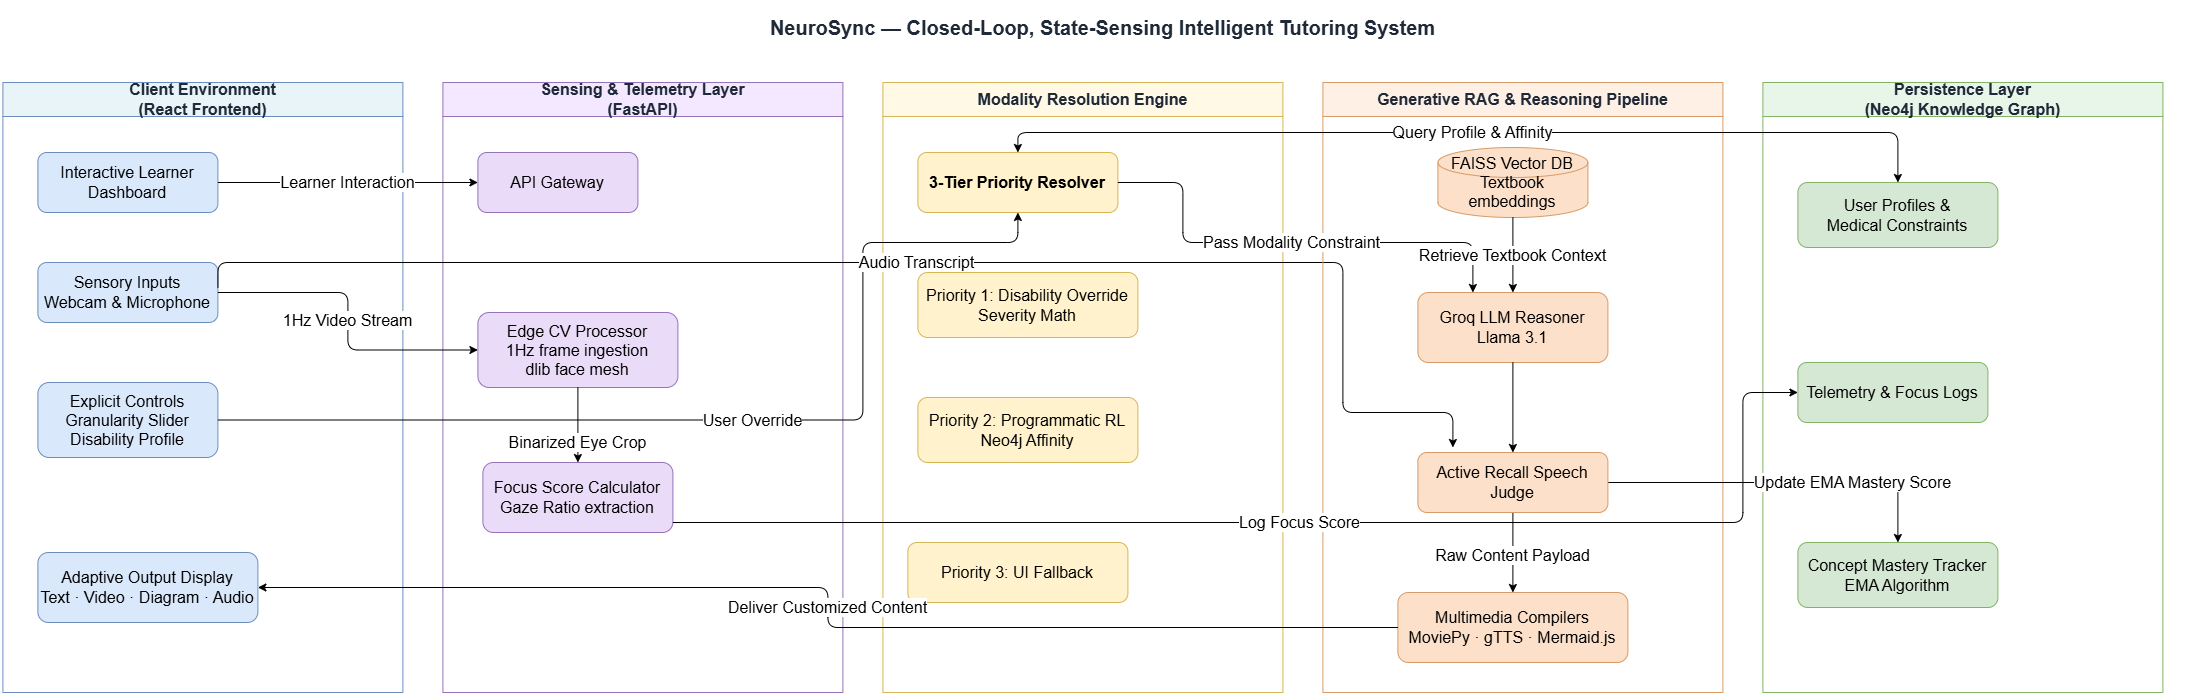
\includegraphics[width=\linewidth]{figures/system_architecture.png}
    \caption{The four-layer closed-loop architecture of the state-sensing ITS.}
    \label{fig:architecture}
\end{figure*}

\subsection{AI Models and Algorithms}
\label{subsec:models_algorithms}

The system processes input queries and learner states through two primary computational engines.

\subsubsection{Adaptive Content Generation Engine}
\label{subsubsec:content_generation_engine}

The content generation engine uses a structured prompt compiler to dynamically format retrieved RAG context. The RAG pipeline retrieves relevant document chunks by minimizing the L2 distance between the embedded query vector $\mathbf{e}_q$ and chunk vectors $\mathbf{e}_c$:
\begin{equation}
    c_i = \arg\min_{c \in \mathcal{C}} \|\mathbf{e}_q - \mathbf{e}_c\|_2^2
\end{equation}
The retrieved chunks are appended to a context prompt. The system classifies the user's query intent into one of five categories: \textit{summarize}, \textit{explain}, \textit{compare}, \textit{analyze}, or \textit{general}. Based on this intent and the resolved modality $M_P \in \{\text{text}, \text{audio}, \text{video}, \text{diagram}\}$, the engine structures its prompt instructions:
\begin{itemize}
    \item \textbf{Text Explanations:} Generates content calibrated to the user-selected Feedback Granularity slider ($0$--$10$) and anxiety level. If anxiety $A \ge 7$, explanations are limited to at most two concepts using simple sentences and comforting reassurance.
    \item \textbf{Diagram Compilation:} The model generates Mermaid.js flowcharts using a strict schema (beginning with \texttt{graph TD;}, terminating lines with \texttt{;}, and using simple node labels) to ensure it compiles correctly on the client interface.
    \item \textbf{Audio Narration:} The model writes conversational explanations, which the server processes into an MP3 file using Google Text-to-Speech (\texttt{gTTS}), bypassing unreliable browser-native synthesis libraries.
    \item \textbf{Video Synthesis:} The LLM generates a structured script containing slide titles, Pexels search keywords, slide bullet points, and voice narration. A background task fetches slide background images from the Pexels API, overlays text using Pillow, generates narration audio via \texttt{gTTS}, and stitches assets into an MP4 file using \texttt{MoviePy} and FFmpeg.
\end{itemize}

\subsubsection{Learner Modeling and Personalization Engine}
\label{subsubsec:learner_modeling_engine}

This engine maintains the student's cognitive state and updates the Neo4j Knowledge Graph.

\begin{enumerate}
    \item \textbf{Real-Time Eye Tracking \& Focus Sessions (Client-Capture, Backend-Analyze):} The React frontend accesses the webcam and uses a hidden \texttt{<canvas>} element to capture and compress a frame every second ($1\text{ Hz}$). This frame is streamed as a base64 string to the FastAPI backend.
    
    The Python backend decodes the frame and utilizes \texttt{dlib} with the pre-trained \texttt{shape\_predictor\_68\_face\_landmarks.dat} model to map facial landmarks. Let $I_{\text{eye}}(x,y)$ be the grayscale image of an eye region. The region is binarized using a threshold of $70$:
    \begin{equation}
        B_{\text{eye}}(x,y) = \begin{cases} 255 & \text{if } I_{\text{eye}}(x,y) < 70 \\ 0 & \text{otherwise} \end{cases}
    \end{equation}
    The binarized eye crop is split horizontally into left ($L$) and right ($R$) halves. The gaze ratio $G$ is defined as the ratio of white pixels in each half:
    \begin{equation}
        G = \frac{\sum_{(x,y) \in L} \mathbb{1}(B_{\text{eye}}(x,y) == 255)}{\sum_{(x,y) \in R} \mathbb{1}(B_{\text{eye}}(x,y) == 255)}
    \end{equation}
    A frame is classified as \textit{attended} if $0.5 \le G \le 2.0$. The session focus score is calculated as the percentage of attended frames:
    \begin{equation}
        S_{\text{focus}} = \frac{N_{\text{attended}}}{N_{\text{total}}} \times 100
    \end{equation}
    The resulting attention score is logged directly to Neo4j. This architecture ensures heavy computer vision processing stays on the server while scaling smoothly across concurrent web users.

    \begin{figure}[htpb]
        \centering
        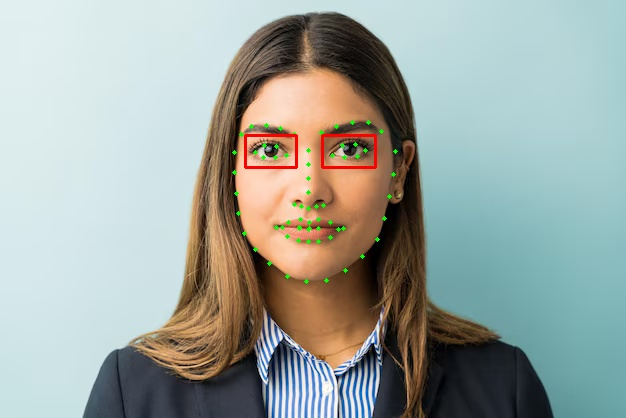
\includegraphics[width=\linewidth]{figures/gaze_pipeline.png}
        \caption{Computer Vision Gaze Tracking Pipeline mapping facial landmarks to binarized eye crops.}
        \label{fig:gaze_pipeline}
    \end{figure}

    \item \textbf{Modality Resolution Hierarchy:} When generating responses, the system resolves competing inputs (user selected modality, inferred behavior, and medical profile) through a strict Priority Hierarchy:
    \begin{itemize}
        \item \textbf{Priority 1: Disability Accommodations (Top Override):} Takes absolute precedence over all other preferences. If comorbid conditions exist (e.g., both ADHD and Dyslexia), the dominant condition is isolated using a two-step formula:
        \begin{equation}
        \begin{split}
            \text{DominantCondition} = \arg\max_{c \in D} \Big( \text{SeverityWeight}(c)\\ +  \epsilon \cdot \text{TieBreakerRank}(c) \Big)
            \end{split}
        \end{equation}
        where $\text{SeverityWeight}(c) \in \{\text{Severe}=3, \text{Moderate}=2, \text{Mild}=1\}$, and $\epsilon = 0.1$ acts as a small weight ensuring the rank only breaks ties without overriding primary severity. Equal severities are resolved using a hardcoded pedagogical tie-breaker matrix: $\text{Dyslexia} > \text{Autism} > \text{ADHD}$. Once isolated, it maps to a scientifically backed modality (e.g., Severe ADHD $\rightarrow$ Diagram, Mild Dyslexia $\rightarrow$ Audio).
        
        \item \textbf{Priority 2: Behavioral Inference (Programmatic RL Loop):} If no disabilities are declared, the system checks for an \texttt{observed\_modality} determined by engagement frequencies in Neo4j. Modality interaction count ($N_{\text{usage}}$) acts as the reward signal. The policy selects the modality with the highest affinity $\theta_u(M)$:
        \begin{equation}
            \theta_u(M) = N_{\text{usage}}(M)
        \end{equation}
        If the system infers via \texttt{infer\_preferred\_modality} and \texttt{get\_modality\_affinity} that the user spends significantly more time engaging with a specific modality (e.g., watching videos), it assumes implicit behavior is a better indicator of learning style than manual choice, overriding the default.
        
        \item \textbf{Priority 3: User Selected Modality (Fallback):} Falls back to the explicit dropdown choice (\texttt{user\_modality}) if no medical constraints or historical behavioral data exist.
    \end{itemize}

    \begin{figure}[htpb]
        \centering
        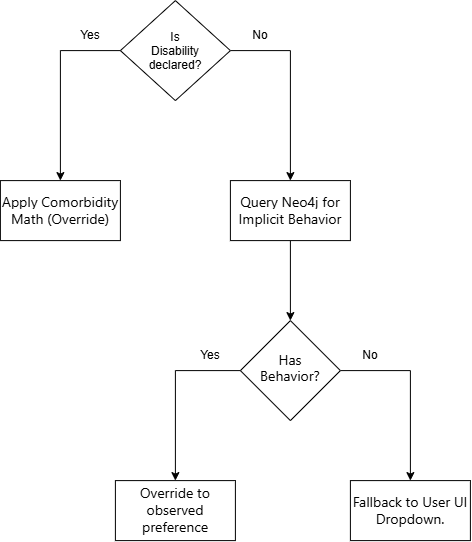
\includegraphics[width=\linewidth]{figures/modality_decision_tree.png}
        \caption{3-Tier Priority Hierarchy for Modality Resolution.}
        \label{fig:modality_hierarchy}
    \end{figure}

    \item \textbf{Rethinking Reinforcement Learning (Programmatic Feedback Loops):} While traditional machine learning RL models (e.g., PPO or Q-learning) are computationally expensive and risk optimization alignment failures (such as optimizing for view time by suggesting highly distracting videos even if they hurt learning), our system implements a **Programmatic Behavioral Inference Loop** using Neo4j analytics. The environment is the chat interface, the action is the modality selection, the reward signal is interaction duration logged as \texttt{ModalityEvents}, and the policy update queries Neo4j to update future defaults. This achieves the autonomous personalization benefits of RL while maintaining 100\% control, transparency, and safety for neurodivergent learners.

    \item \textbf{Pedagogical Logic and Disability Accommodations:}
    The system maps verified clinical principles directly to generative constraints, as summarized in Table~\ref{tab:accommodations}.
    \begin{table*}[htpb]
        \centering
        \caption{Pedagogical Accommodations Matrix}
        \label{tab:accommodations}
        \resizebox{\linewidth}{!}{%
        \begin{tabular}{llll}
            \toprule
            \textbf{Disability Profile} & \textbf{Theoretical Framework} & \textbf{ITS System Action} & \textbf{Generated Modality} \\
            \midrule
            ADHD & Cognitive Load Theory & Limits concepts, bulleted points & Video / Diagram \\
            ASD & Visual Support Theory & Explicit step-by-step logic, no idioms & Diagram \\
            Dyslexia & Orton-Gillingham & Simple vocabulary, phonetic support & Audio (TTS) \\
            \bottomrule
        \end{tabular}%
        }
    \end{table*}
    
    \item \textbf{Learner Autonomy (Feedback Granularity \& Anxiety):} 
    Rather than forcing a fixed explanation depth, the frontend provides a manual \textit{Feedback Granularity} slider ($0$--$10$). This empowers students with explicit control over their cognitive load, allowing them to choose surface-level bite-sized summaries (low granularity) or deep technical breakdowns (high granularity) depending on their current mental bandwidth.
\end{enumerate}

\subsection{User Interface and Accessibility Design}
\label{subsec:ui_accessibility}

The frontend is built using React and Material-UI, following Web Content Accessibility Guidelines (WCAG 2.1). 
Key accessibility features include:
\begin{itemize}
    \item \textbf{Visual Styling:} High-contrast dark and light modes using system preference fallbacks, featuring a fluid glassmorphism layout with legible typography (Inter and Outfit) for dyslexic readers.
    \item \textbf{Speech Evaluation Interface:} An active speech loop using the browser's \texttt{webkitSpeechRecognition} API. It allows students to explain concepts in their own words. The system transcribes the speech and evaluates understanding against the RAG reference text.
    \item \textbf{Comprehension Scaffolding:} Action buttons (\textit{Understood} and \textit{Not Understood}) let students self-regulate. Clicking \textit{Understood} generates an adaptive MCQ quiz, while \textit{Not Understood} automatically simplifies the concept.
\end{itemize}

\subsection{Data Privacy and Security Considerations}
\label{subsec:privacy_security}

Given the use of webcam data and personal cognitive profiles, the system implements a strict privacy-preserving model:
\begin{itemize}
    \item \textbf{Local Eye-Tracking Processing:} Gaze ratio calculation is processed in-memory at the FastAPI application layer. Individual camera frames are analyzed on-the-fly and immediately discarded. No video files or raw frames are saved or transmitted outside the server environment.
    \item \textbf{Granular User Consents:} The system requires explicit user consent before activating the webcam or using declared cognitive profiles (ADHD, ASD, Dyslexia) for personalization.
    \item \textbf{Data Deletion Policies:} In line with GDPR requirements, users can delete their profiles. The interface provides a "Delete My Data" feature that performs a cascading detach-delete on the Neo4j database, removing all related sessions, masteries, focus scores, and interaction logs.
\end{itemize}

\section{Implementation Details}
\label{sec:implementation}

This section describes the development environment, package dependencies, and a step-by-step walk-through of the prototype interface.

\subsection{Development Environment and Tools}
\label{subsec:dev_environment}

The system is split into a frontend web client and a backend API server:
\begin{enumerate}
    \item \textbf{Frontend Development Stack:} 
    \begin{itemize}
        \item \textbf{Core Library:} React.js with Material-UI (MUI) for responsive design and theme configuration.
        \item \textbf{Data Visualisation:} Recharts for rendering focus dashboard charts, and Mermaid.js for drawing live vector flowcharts.
        \item \textbf{Speech Processing:} The HTML5 Web Speech API (\texttt{webkitSpeechRecognition}) for transcribing user answers.
        \item \textbf{Audio Management:} Howler.js for playing, pausing, and repeating audio voiceovers.
        \item \textbf{Network Communication:} Axios for handling REST API requests to the FastAPI backend.
    \end{itemize}
    
    \item \textbf{Backend Development Stack:}
    \begin{itemize}
        \item \textbf{Framework:} FastAPI with Uvicorn acting as the server gateway.
        \item \textbf{Cognitive Reasoning \& RAG:} The Groq Python SDK connecting to the \texttt{llama-3.1-8b-instant} model; \texttt{sentence-transformers} (\texttt{all-MiniLM-L6-v2}) for generating embeddings; and \texttt{faiss-cpu} for vector indexing.
        \item \textbf{Local NLP Processing:} Hugging Face \texttt{transformers} running local models for summary extraction (\texttt{facebook/bart-large-cnn}) and named entity recognition (\texttt{dslim/bert-base-NER}).
        \item \textbf{Computer Vision:} OpenCV (\texttt{opencv-python}) for image decoding and dlib for facial landmark tracking, using the pre-trained \texttt{shape\_predictor\_68\_face\_landmarks.dat} dataset.
        \item \textbf{Multimedia Synthesis:} MoviePy and FFmpeg for compiling video slides, gTTS for generating speech, and PyMuPDF (\texttt{fitz}) for extracting text from uploaded PDFs.
        \item \textbf{Database Driver:} The official \texttt{neo4j} Python driver for connecting to a cloud-hosted Neo4j instance.
    \end{itemize}
\end{enumerate}

\subsection{Prototype Walkthrough and Use Cases}
\label{subsec:walkthrough_usecases}

The prototype workflow is illustrated through a representative learning scenario:
\begin{enumerate}
    \item \textbf{Profile Initialization \& Comorbidity Strategy Setup:}
    A student starts by creating a profile (e.g., ``Username1''). The system registers a new \texttt{User} node in Neo4j with a unique ID via the \texttt{/create-profile} endpoint. The student consents and declares two comorbid conditions in the Sidebar: moderate ADHD and moderate Dyslexia. Since both conditions have equal severity ($\text{weight}=2$), the priority resolution engine evaluates Eq. (5), selecting Dyslexia as the dominant condition and triggering the Audio modality to support phonological decoding.
    
    \item \textbf{Study Material Upload \& Query:}
    The student uploads a computer science PDF textbook. The server extracts the text, creates vector embeddings for 300-word segments, and loads them into a FAISS index. The student types a question: \textit{``What is cloud computing?''}.
    
    \item \textbf{Active Gaze Tracking \& Telemetry:}
    The student clicks \texttt{Start Session}, granting camera access. The browser streams base64 frame captures to the server at $1\text{ Hz}$. While reading the material, if the student shifts their gaze away from the screen, the gaze-tracking engine calculates an out-of-bounds ratio and logs a distracted state. If the student scrolls frantically or clicks repeatedly, the client-side system detects this impatience, logs it in Neo4j, and shows a mindfulness prompt to help them refocus.
    
    \item \textbf{Adaptive Content Delivery \& Programmatic RL Logging:}
    The FastAPI server processes the query, retrieves textbook context using FAISS, and identifies the student's declared ADHD profile. It overrides the default text modality and instructs the LLM to output a visual Mermaid flowchart showing client-server cloud relationships. The client renders the flowchart, allowing the student to zoom, view it in full screen, or download it as an SVG.
    As the student interacts with the visual chart, the system records interaction frequencies, logging a \texttt{ModalityEvent} to Neo4j. This forms the reward signal that updates the programmatic feedback loop for future queries.
    
    \item \textbf{Active Comprehension Verification:}
    \begin{itemize}
        \item \textbf{RAG Quiz Verification:} The student clicks \texttt{Understood}. The backend generates a 3-question MCQ quiz based on the retrieved context. The student answers the questions, and the server calculates a score, explains any errors, and saves the mastery levels to Neo4j.
        \item \textbf{Active Recall Speech Check:} Alternatively, the student clicks \texttt{Explain what you know} and explains the concept aloud. The Web Speech API captures and transcribes their voice, sending it to the server. The LLM acts as an automated judge via a dedicated prompt, computing the semantic alignment between the transcribed student response and the source RAG context. It returns a binary Pass/Fail verification alongside constructive feedback, ensuring deep conceptual construction rather than passive recall.
    \end{itemize}
\end{enumerate}

\section{Evaluation and Results}
\label{sec:evaluation}

Evaluating a state-sensing Generative AI Intelligent Tutoring System (ITS) presents unique challenges due to the non-deterministic nature of large language models and the complex integration of multi-modal telemetry. To address this, the evaluation of the proposed framework is divided into two parts: an empirical verification of system integrity and pedagogical logging currently active in the codebase, and a roadmap of automated telemetry reserved for future production releases.

\subsection{Concept Mastery Tracking Evaluation}
\label{subsec:eval_mastery}

To measure pedagogical efficacy, the system tracks student information retention and mastery over time. The primary evaluation metric is the student's performance on adaptive quizzes generated dynamically from the Retrieval-Augmented Generation (RAG) textbook context. 

When a student completes an evaluation quiz, the server processes their response accuracy and updates a persistent \texttt{HAS\_MASTERY} relationship in the Neo4j knowledge graph. To avoid high volatility from isolated attempts, the database computes an exponential moving average (EMA) of the mastery level. Let $S_k$ be the updated mastery score after the $k$-th quiz attempt, and $S_{\text{quiz}} \in [0, 1]$ be the score of the current quiz submission. The mastery score is updated recursively as follows:
\begin{equation}
    S_k = 0.7 \cdot S_{k-1} + 0.3 \cdot S_{\text{quiz}}
\end{equation}
where $S_0 = 0$. This updating formula ensures that long-term mastery trends are prioritized while still accounting for recent performance. 

\begin{figure}[htpb]
    \centering
    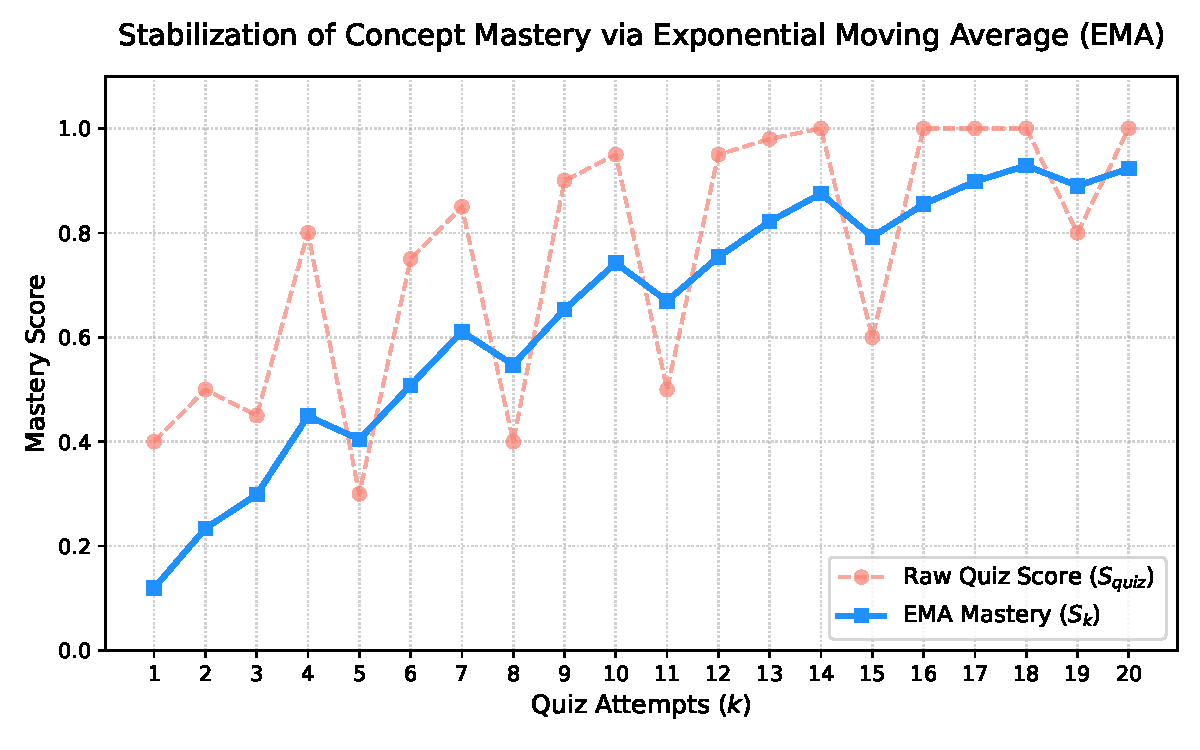
\includegraphics[width=\linewidth]{figures/ema_mastery_trend.pdf}
    \caption{Stabilization of Concept Mastery via Exponential Moving Average (EMA) smoothing.}
    \label{fig:ema_mastery}
\end{figure}

Administrators and educators can track individual student trendlines over time through the system's interactive frontend dashboard. The React client dynamically fetches these calculated mastery records via REST API endpoints and renders them as comprehensive visual charts using Recharts, providing direct, accessible empirical evidence of the tutoring system's educational impact.

\subsection{Behavioral Adaptation Evaluation}
\label{subsec:eval_behavioral}

The evaluation of the behavioral adaptation loop verifies whether the system correctly gathers interaction metadata and adapts content to inferred user habits. The system tracks user interactions by logging a \texttt{ModalityEvent} relationship to the graph whenever the learner engages with a specific medium (e.g., text, audio, video, or diagram).

The efficacy of the behavioral loop is validated by querying the relationship count of the \texttt{USES} edge connected to the \texttt{ObservedModality} nodes in the graph database. Because modality adaptations rely on interaction counts to determine preference, verifying the loop involves monitoring whether the Cypher query-based recommendation algorithm updates user preferences under different interaction scenarios. By checking if the backend successfully overrides the default text output with diagrams or audio once a specific threshold of interaction counts is exceeded, we verify that the programmatic reinforcement loop functions dynamically and predictably without requiring heavy neural-network policy optimizations. Additionally, these behavioral logs and modality affinities are fed into the user's dashboard interface, providing transparent visual representations of how their interactions directly govern the system's delivery strategies.

\subsection{Database Integrity Verification}
\label{subsec:eval_integrity}

In the initial release of this state-sensing prototype, functional validation is performed through live database integrity checks rather than mock test suites. This verification ensures that data streams from separate sensing pipelines—such as computer vision gaze scores and micro-interaction scroll/click events—are accurately processed and stored.

Database integrity is verified by executing live Cypher queries directly on the Neo4j instance during active study sessions. A representative verification query is shown below:
\begin{verbatim}
MATCH (u:User)-[r:HAS_FOCUS_SESSION]->(f:FocusSession)
RETURN u.user_id, r, f.score, f.label
\end{verbatim}

\begin{figure}[htpb]
    \centering
    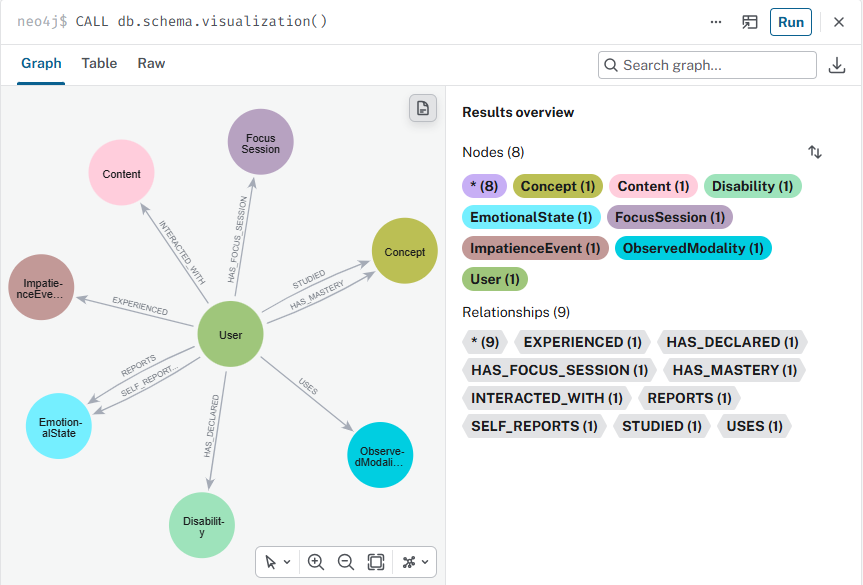
\includegraphics[width=\linewidth]{figures/neo4j_schema.png}
    \caption{Neo4j Knowledge Graph Schema illustrating Nodes and pedagogical Relationships.}
    \label{fig:neo4j_schema}
\end{figure}

By querying the graph in real-time, we verify that:
\begin{itemize}
    \item The eye-tracking focus scores generated at $1\text{ Hz}$ by the OpenCV/dlib engine are aggregated correctly and saved with the appropriate classification label (e.g., "High Focus" or "Moderate Focus"). These data points are subsequently relayed to the frontend dashboard, where focus trendlines are plotted visually using Recharts to provide students and educators with an immediate snapshot of session-by-session attention spans.
    \item Gaze and micro-interaction telemetry are strictly mapped to the active \texttt{user\_id}, confirming database boundary security and preventing data leaks in multi-user settings.
\end{itemize}

\subsection{Future Evaluation Directions}
\label{subsec:eval_future}

To transition the platform from a functional research prototype to an enterprise-grade production application, several evaluation metrics and automated pipelines are planned for integration:
\begin{itemize}
    \item \textbf{Automated Latency Telemetry:} Future iterations will implement background performance timers to track execution latency. This will capture the millisecond duration of the RAG vector search, LLM text generation, and the MoviePy video compiling pipeline, allowing developers to identify bottleneck points.
    \item \textbf{Continuous Integration (CI) Compilation Tests:} Setting up automated testing suites using frameworks like \texttt{pytest} and \texttt{jest}. These suites will run regular mock prompts to verify that the LLM-generated Mermaid.js syntax compiles correctly without rendering errors on the client interface.
    \item \textbf{UI/UX and Attention Survey Correlation:} Upgrading the current user feedback modal to actively collect subjective evaluations. Students will rate the perceived accuracy of their focus scores, the readability of the glassmorphism UI, and overall learning satisfaction. These responses will be stored directly in Neo4j to correlate objective attention metrics with subjective student experiences.
\end{itemize}

\section{Discussion}
\label{sec:discussion}

The development and initial evaluation of the proposed state-sensing Intelligent Tutoring System (ITS) offer critical insights into the intersection of Generative AI, affective computing, and neurodiversity-oriented educational technology. This section analyzes the pedagogical and database verification results, explores the broader social and educational implications, and addresses the technical limitations of the current prototype.

\subsection{Analysis of Results}
\label{subsec:analysis_results}

The initial evaluation of the prototype validates three core aspects of the system design: the stabilization of the concept mastery tracking loop, the reliability of the programmatic modality adaptation loop, and the integrity of the real-time telemetry pipeline.

First, the integration of an Exponential Moving Average (EMA) for updating student mastery scores represents a significant advancement over static, transaction-based knowledge tracking. Traditional tutoring systems often exhibit high volatility in performance metrics; a student's temporary lapse in attention or a poorly timed distraction can lead to low quiz scores, triggering premature and frustrating pedagogical remediation. The $0.7$ history-smoothing coefficient in Eq. (7) ensures that isolated quiz failures do not derail overall learning progress, while still maintaining responsiveness to persistent declines in comprehension. Crucially, representing this stabilized trendline on the React dashboard via Recharts provides encouraging visual feedback, which educational psychology links to reduced test anxiety and enhanced metacognitive self-regulation.

Second, the programmatic reinforcement loop offers a robust, predictable alternative to complex, neural-network-based reinforcement learning (RL). Deep RL algorithms (e.g., PPO or DQNs) require massive datasets, introduce alignment risks (such as optimizing for view time over learning depth), and operate as black boxes. By contrast, tracking \texttt{USES} interaction counts in Neo4j keeps the system transparent, auditable, and computationally lightweight. Furthermore, the FastAPI backend enforces clinical compliance by placing verified medical accommodations strictly above behavioral patterns in the priority hierarchy.

Third, real-time database verification via Cypher queries demonstrated that the $1\text{ Hz}$ gaze-tracking telemetry is accurately parsed and bound to the active \texttt{user\_id}. The system successfully distinguishes between active cognitive engagement (marked by steady gaze ratios and moderate scroll frequencies) and mechanical frustration (characterized by rapid scrolling, repetitive clicks, and low gaze ratios). By relaying these focus scores to the frontend, Recharts visualizes focus trendlines session-by-session, validating the database integration and providing students with a transparent window into their own attention patterns.

\subsection{Social Impact and Educational Implications}
\label{subsec:social_impact_implications}

The proposed closed-loop state-sensing tutor has profound implications for educational equity, cognitive accessibility, and the design of learner-centered environments.

From an equity perspective, specialized education for neurodivergent learners—such as those with ADHD, Autism, or dyslexia—is often highly resource-intensive. Families must rely on specialized tutors, clinical therapists, or expensive private schooling, creating a severe socioeconomic divide in academic achievement. By integrating Universal Design for Learning (UDL) guidelines, Visual Support Theory, and Orton-Gillingham reading principles directly into a digital platform, this architecture democratizes access to personalized accommodations. Any student with a basic webcam and internet access can leverage a state-sensing tutoring environment that adapts content structures (e.g., visual Mermaid.js flowcharts for dyslexic/ASD profiles or audio narration for orthographic decoding bottlenecks) without requiring specialized hardware or manual intervention.

Furthermore, this system prompts a shift from ``answer engines'' to true pedagogical scaffolding. The widespread deployment of standard LLM interfaces in education has led to concerns that GenAI acts as a shortcut, where students copy-paste answers to bypass cognitive effort. The active recall speech check (using the Web Speech API) and the RAG-driven adaptive quizzes force students into active cognitive construction. By requiring verbal explanations or conceptual verification before updating the \texttt{HAS\_MASTERY} relationships, the system enforces deep conceptual processing, shifting the role of AI from a passive oracle to an active conversational tutor.

Finally, the project demonstrates that affective computing can be implemented in a privacy-preserving manner. In an era of surveillance capitalism, educational tools often harvest student biometric data, raising severe ethical and security concerns. The system's architecture calculates eye-tracking metrics entirely in-memory at the FastAPI layer, immediately discarding raw image frames. By combining this local processing with a GDPR-compliant cascading detach-delete function in Neo4j, the system establishes a precedent for trust, proving that real-time state adaptation and biometric feedback do not require the central archiving of sensitive personal data.

\subsection{Limitations of the Current Prototype}
\label{subsec:limitations_prototype}

Despite its functional capabilities, the current prototype is subject to several technical and clinical limitations that represent opportunities for future research:
\begin{enumerate}
    \item \textbf{Sensitivity of Edge-Based Eye Tracking:} Gaze ratio estimation is highly dependent on ambient environmental conditions. Low lighting, backlighting, sudden head movements, and light reflections on eyeglasses can distort the dlib landmark coordinates. This leads to false-positive distraction classifications. Furthermore, running dlib's 68 facial landmark detector on a single CPU thread can lead to processing overhead and frame drops on lower-end consumer laptops.
    \item \textbf{High Computational Latency of Video Synthesis:} Generating customized educational videos represents a major performance bottleneck. Compiling video slide-decks using MoviePy, Pillow, gTTS, and FFmpeg is a synchronous, CPU-bound task. For students with severe ADHD who require video-based delivery, the $10$--$15$ second delay required to compile slides, synthesize audio voiceovers, and write text layers disrupts the flow of conversational learning, introducing conversational lag.
    \item \textbf{LLM Hallucinations in Syntax Compilation:} The diagram generation engine relies on Llama 3 to output structured Mermaid.js flowchart syntax. Despite strict prompt compilation rules, the non-deterministic nature of LLMs occasionally results in minor syntax errors (e.g., nested parentheses, unmatched brackets, or forbidden node labeling characters). When these errors occur, the React client's Mermaid renderer fails, displaying a blank container instead of the visual flowchart.
    \item \textbf{Absence of Longitudinal Clinical Studies:} The validation presented in this work is restricted to database integrity verification and functional loop testing. The prototype has not yet been deployed in a longitudinal, clinical, or classroom-based study. Consequently, while the EMA mastery trendlines and modality transition counts stabilize programmatically, we cannot yet empirically confirm that this closed-loop adaptation results in superior long-term recall, increased working memory capacity, or reduced academic anxiety compared to standard static text tutoring.
\end{enumerate}

\section{Conclusion and Future Work}
\label{sec:conclusion}

This paper has presented a state-sensing, closed-loop Intelligent Tutoring System (ITS) designed to address the cognitive, affective, and sensory requirements of neurodivergent learners. By integrating real-time telemetry streams with generative models and a graph-based learner profile, the system shifts the adaptive tutoring paradigm from simple text adjustments to dynamic, multimodal content scaffolding.

\subsection{Summary of Contributions}
\label{subsec:summary_contributions}

In summary, this research advances adaptive educational technology through four primary milestones: (1) a privacy-by-design sensing pipeline that captures focus and impatience in-memory without storing raw biometric video; (2) a dynamic multimodal engine that compiles textbook context into diagrams, audio streams, and videos; (3) a neurodiversity-first priority hierarchy in Neo4j that deterministically resolves comorbid accommodations; and (4) an active recall verification loop that transforms GenAI from a passive answer engine into an active, state-sensing tutor.

\subsection{Future Work}
\label{subsec:future_work}

To overcome the current limitations of the prototype and expand the system's capabilities, several future research and development directions are proposed:
\begin{enumerate}
    \item \textbf{Transition to Client-Side GPU Telemetry:} The sensitivity and processing overhead of backend eye tracking can be resolved by migrating the gaze-estimation pipeline to the client browser. Leveraging WebAssembly and WebGL-based facial landmark libraries (such as MediaPipe FaceMesh) will enable $30\text{ Hz}$ gaze tracking executed directly on the user's local GPU context. This eliminates base64 frame-streaming latency, reduces backend server compute costs, and ensures raw camera inputs never leave the client device.
    \item \textbf{Optimized Multimedia Synthesis and Streaming:} To eliminate the $10$--$15$ second delay in generating MoviePy educational videos, the backend compilation pipeline can be optimized using asynchronous task queues (e.g., Celery with Redis). Furthermore, the frontend can transition from static video file downloads to rendering interactive canvas-based animations or vector slides dynamically on the fly, transforming text segments into interactive slides without rendering full video files.
    \item \textbf{Grammar-Constrained Syntax Parsing:} To prevent Mermaid.js flowchart rendering failures, future iterations will integrate schema-enforcing decoding libraries (such as Outlines or Guidance) on the LLM backend. By forcing the language model's logit generation to conform strictly to a Mermaid context-free grammar, syntax compilation errors will be mathematically eliminated. Additionally, an Abstract Syntax Tree (AST) validator on the backend will inspect diagrams prior to transmission, prompting an automated self-correction loop if any syntax deviations occur.
    \item \textbf{Controlled Longitudinal Classroom Evaluations:} To validate the pedagogical efficacy of the Exponential Moving Average (EMA) mastery updates and modality selection models, we plan to execute a controlled, double-blind clinical study with neurodivergent students. This evaluation will track time-to-mastery, cognitive load (via NASA-TLX surveys), and student retention rates over a multi-month curriculum to empirically correlate real-time telemetry adaptations with academic performance improvements.
    \item \textbf{Affective Sensing and Multi-Agent Expansion:} The telemetry input channel will be expanded to detect emotional states (such as frustration, confusion, or boredom) by integrating facial micro-expression classifiers (e.g., DeepFace) and voice sentiment analysis during speech checks. Additionally, the reasoning layer will be restructured into a collaborative multi-agent framework, deploying specialized agent personas (e.g., a Socratic tutor, a visual translator, and an emotional support agent) that coordinate to manage the student's learning session.
\end{enumerate}

\section*{References}
\begin{thebibliography}{99}

\bibitem{1}
Jurenka, I., Kunesch, M., McKee, K. R., Gillick, D., Zhu, S., Wiltberger, S., ... \& Ibrahim, L. (2025). Towards Responsible Development of Generative AI for Education: An Evaluation-Driven Approach. \textit{arXiv preprint arXiv:2407.12687}.

\bibitem{2}
Laak, K. J., \& Aru, J. (2025). AI and personalized learning: bridging the gap with modern educational goals. \textit{arXiv preprint arXiv:2404.02798}.

\bibitem{3}
Vorobyeva, K. I., Belous, S., Savchenko, N. V., Smirnova, L. M., Nikitina, S. A., \& Zhdanov, S. P. (2025). Personalized learning through AI: Pedagogical approaches and critical insights. \textit{Contemporary Educational Technology}, 17(2), Article ep574. \url{https://doi.org/10.30935/cedtech/16108}

\bibitem{4}
Binhammad, M., Othman, A., Abuljadayel, L., Mheiri, H., Alkaabi, M., \& Almarri, M. (2024). Investigating How Generative AI Can Create Personalized Learning Materials Tailored to Individual Student Needs. \textit{Creative Education}, 15(7), pp. 1499--1523. \url{https://doi.org/10.4236/ce.2024.157091}

\bibitem{5}
Vijayasekaran, G., Bibiana, J. J., Sankeerthana, D., Soumya, K., Hema, D., \& Kusuma, B. (2024). Personalized Learning Platform using Artificial Intelligence. In \textit{2024 9th International Conference on Communication and Electronics Systems (ICCES)} (pp. 1883--1890). IEEE. \url{https://doi.org/10.1109/ICCES63552.2024.10859816}

\bibitem{6}
Sarkar, S., S, R., R, G., M, J., \& Kudiyarasu, J. (2025). Generative AI for Personalized Learning Experiences in Education. In \textit{2025 International Conference on Computing and Communication Technologies (ICCCT)} (pp. 1--15). IEEE. \url{https://doi.org/10.1109/ICCCT63501.2025.11020445}

\bibitem{7}
Abbes, F., Bennani, S., \& Maalel, A. (2024). Generative AI and Gamification for Personalized Learning: Literature Review and Future Challenges. \textit{SN Computer Science}, 5(8), Article 1154. \url{https://doi.org/10.1007/s42979-024-03491-z}

\bibitem{8}
JIER Research Group (2025). AI in Personalized Learning and Educational Assessment. \textit{Journal of Informatics Education and Research}, 5(2), pp. 45--58. \url{https://doi.org/10.52783/jier.v5i2.2688}

\bibitem{9}
Singh, A. (2024). Investigating the Use of Generative AI for Creating Personalized Learning Paths Tailored to Individual Students' Cognitive Needs. \textit{SSRN Electronic Journal}. \url{https://doi.org/10.2139/ssrn.5194545}

\bibitem{10}
Pesovski, I., Santos, R., Henriques, R., \& Trajkovik, V. (2024). Generative AI for Customizable Learning Experiences. \textit{Sustainability}, 16(7), Article 3034. \url{https://doi.org/10.3390/su16073034}

\bibitem{11}
Morales-Chan, M., Amado-Salvatierra, H. R., \& Hernandez-Rizzardini, R. (2024). AI-Driven Content Creation: Revolutionizing Educational Materials. In \textit{Proceedings of the Eleventh ACM Conference on Learning @ Scale} (pp. 556--558). \url{https://doi.org/10.1145/3657604.3664640}

\bibitem{12}
Admane, R., Sawale, P. S., Jayasree, R., Kurup, S. J., \& Thomas, S. A. (2024). Artificial Intelligence in Education: Tailoring Curriculum to Individual Student Needs through AI-Based Systems. \textit{Library of Progress-Library Science, Information Technology \& Computer}, 44(3), pp. 8847--8858.

\bibitem{13}
Farhah, N. S., Wadood, A., \& Alqarni, A. A. (2025). Enhancing Adaptive Learning with Generative AI for Tailored Educational Support for Students with Disabilities. \textit{Journal of Disability Research}, 4(3), Article JDR-2025-0012. \url{https://doi.org/10.57197/JDR-2025-0012}

\bibitem{14}
Krouska, A., Troussas, C., Voyiatzis, I., Mylonas, P., \& Sgouropoulou, C. (2024). ChatGPT-based Recommendations for Personalized Content Creation and Instructional Design with a Tailored Prompt Generator. In \textit{2024 2nd International Conference on Foundation and Large Language Models (FLLM)} (pp. 295--299). IEEE. \url{https://doi.org/10.1109/FLLM63129.2024.10852487}

\bibitem{15}
Yusri, A. B. (2024). Speed reading tool powered by artificial intelligence for students with ADHD, dyslexia, or short attention span (Technical Report). \textit{Computational Intelligence, Universiti Teknologi Malaysia}, Johor Bahru, Malaysia.

\bibitem{16}
Rocha, V., Queiroz, J., \& Silva, C. (2025). An AI Gen and LLM-Based Platform for Pedagogical Support and Sensory Accommodations for Neurodivergent Students. In \textit{Proceedings of the 21st Brazilian Symposium on Information Systems} (pp. 231--240). SBC. \url{https://doi.org/10.5753/sbsi.2025.246443}

\bibitem{17}
Hamzaoui, H., Bachiri, M., Ouassam, A., Mouncif, H., \& Bouikhalene, B. (2024). Toward Artificial Intelligence-Enhanced Hybrid Learning: Leveraging Video Content for Personalized Education. In \textit{Proceedings of the 7th International Conference on Networking, Intelligent Systems and Security (NISS '24)}. ACM. \url{https://doi.org/10.1145/3659677.3659823}

\bibitem{18}
Mittal, U., Sai, S., Chamola, V., \& Sangwan, D. (2024). A Comprehensive Review on Generative AI for Education. \textit{IEEE Access}, 12, pp. 142733--142759. \url{https://doi.org/10.1109/ACCESS.2024.3468368}

\bibitem{19}
Dao, X. Q., Le, N. B., \& Nguyen, T. M. T. (2021). AI-Powered MOOCs: Video Lecture Generation. In \textit{Proceedings of the 2021 3rd International Conference on Image, Video and Signal Processing (IVSP '21)} (pp. 95--102). ACM. \url{https://doi.org/10.1145/3459212.3459227}

\bibitem{20}
ETR Research Group (2025). Artificial Intelligence as an Effective Tool for Personalized Learning in Modern Education. \textit{Environment. Technology. Resources. Proceedings of the International Scientific and Practical Conference}, 3, pp. 187--194. \url{https://doi.org/10.17770/etr2025vol3.8534}

\bibitem{21}
Almetnawy, H., Orabi, A., Alneyadi, A. R., Ahmed, T., \& Lakas, A. (2025). An Adaptive Intelligent Tutoring System Powered by Generative AI. In \textit{2025 IEEE Global Engineering Education Conference (EDUCON)} (pp. 1--10). IEEE. \url{https://doi.org/10.1109/EDUCON62633.2025.11016362}

\bibitem{22}
Leon, M. (2024). Leveraging Generative AI for On-Demand Tutoring as a New Paradigm in Education. \textit{International Journal on Cybernetics \& Informatics (IJCI)}, 13(5), pp. 17--29. \url{https://doi.org/10.5121/ijci.2024.130502}

\end{thebibliography}

\end{document}
